%
% Section 4: Interpretation
%
%   # of slides: 6 (new 10-20!) 
%
% -------------------------------------------------------------------------------
\section{Toy Model Interpretation}
\label{sec:interpret}

\begin{frame}
\frametitle{Interpreting the Toy Model}

Toy model expresses \enskip 
$\Var(T) = \mcal{F}\big(\Var(F_0),\Var(P),\,\text{\tmcoeffs}\big)$

\vspace*{1em}

\begin{itemize}

% Q for coefficients -- mean state
\boxitem[0.88][<1->]{%
%
\textcolorbf{colone}{Q:} \quad
%
\parbox{0.68\linewidth}{\centering
Do the \tmcoeffs \\ show dependence \\ on mean-state variables ? }
%
\uncover<2->{\quad \textcolorbf{colone}{Not today!} } }

% Q for relative contribution of forcing to variance
\boxitem[0.88][<1->]{%
%
\textcolorbf{colone}{Q:} \quad
%
\parbox{0.68\linewidth}{\centering
What are the relative contributions \\ 
of $\Var(F_0)$ and $\Var(P)$ to $\Var(T)$ ?}
%
\uncover<2->{\quad \textcolorbf{colone}{Not today!} } }

% Q for role of land-surface on Var(T)
\boxitem[0.88][<2->]{%
%
\textcolorbf{colone}{Q:} \quad
%
\parbox{0.8\linewidth}{\centering\textcolorbf{colone}{%
What is the role of soil moisture \\ 
(mean-state and anomalies) on $\Var(T)$ ?} } }

\end{itemize}

\end{frame}

\begin{frame} 
\frametitle{{\large Role of the land surface on surface temperature variability}}

\vspace*{-1.5em}

\begin{itemize}

\item<1-> Start from the toy model expression for $\Var(T)$: 
%
\begin{equation*}
%
\hspace*{-1em}
%
  \VarTtm = \frac{1}{\gamma^2}\, \Big[ 
  \big( 1-\textcolor{colone}{\lambda}(1-\textcolor{colone}{\chi}) \big)^2 \Var(F_0) + 
  L^2 \big( \alpha(1-\textcolor{colone}{\lambda})+
   \textcolor{colone}{\chi}(1+\alpha\lambda-\beta) \big)^2 \Var(P)
  \Big] 
%
\end{equation*}

\boxitem[0.88][<2->]{%
%
\textcolorbf{colone}{Set} \qquad
%
\parbox{0.75\linewidth}{
\textcolor{colone}{$\chi$} 
  {\small (effects of soil moisture anomalies on $\Var(T)$)} \\
\textcolor{colone}{$\lambda$} 
  {\small (evapotranspiration efficiency)} }
%
\textcolor{colone}{$\displaystyle = 0$} \\[1.5em]
%
\textcolorbf{colone}{To get:} \qquad
$\displaystyle \VarTtm = \gamma\invv \big[ \Var(F_0) + L^2\alpha^2\Var(P) \big]$
}

\boxitem[0.88][<3->]{\textcolorbf{colone}{Define} \enskip 
%
$\dfrac{\gamma^2\Var(T)}{\Var(F)}$ \enskip 
\textcolorbf{colone}{the surface temperature response} }

\end{itemize}

\end{frame}

\begin{frame}
\frametitle{Two regimes {\large of surface temperature variability}}

\begin{center}

\uncover<1>{%
%
\tikzfig{comp_scale_gammaT}{width=\textwidth} }

\tikzitemMark

\end{center}

\begin{tikzpicture}[overlay]

\coordinate (title) at ($(comp_scale_gammaT.north)+(-0.4,0.4)$);
\node[color=colone,font=\bf] at (title) 
  {Surface temperature response $\gamma^2\Var(T)/\Var(F)$};

% - Surface temperature variability
%   land-surface amplified / damped regimes !!!
\tikzitem[<1>]{\parbox{0.8\linewidth}{\centering%
%
The land surface is able to \\
\textcolorbf{colone}{amplify} and \textcolorbf{colone}{damp} \\
surface temperature variability} }

% show comp_scale_gammaT (with and without global mean soil moisture)
\uncover<2->{%
%
\node at (comp_scale_gammaT) 
  {\includegraphics[width=\textwidth]{comp_scale_gammaT_OvGM}} ; }

\tikzitem[<2>]{\parbox{0.8\linewidth}{\centering%
%
Superpose with global mean soil moisture contour: \\[1ex]
\textcolorbf{coltwo}{Dry soils}
(moisture-limited $E$) 
\textcolorbf{coltwo}{amplify $\Var(T)$}, \\
\textcolorbf{coltwo}{Wet soils} 
(energy-limited $E$)
\textcolorbf{coltwo}{damp $\Var(T)$ } } }

\end{tikzpicture}

\end{frame}

\begin{frame}
\frametitle{Interpret: {\large Land-surface amplified / Moisture-limited}}

\vspace*{-1.5em}

\begin{itemize}

\itemDiamond $\lambda\;$: evapotranspiration efficiency 

\itemDiamond $\chi\;$: coupling coefficient (modulates net effect of $m'$ on $T'$)

\end{itemize}

\begin{center}

% input from figures/diagrams
\ifdraft{}{%
%
\resizebox{\linewidth}{!}{\begin{tikzpicture}
%
% Land-surface damped summary diagram. 
%
% ** include 'uncover' tikz commands **
%
% requires the following tikz libraries:
%   arrows, calc, decorations.pathmorphing, shapes
% 
%   and the 'wasysym' package
% -----------------------------------------------------------------------------

%% Styles and colors

% Color definition (requires \usepackage[svgnames]{xcolor})
\colorlet{sfc}{colone}
\colorlet{landatm}{gray!20!white}
\colorlet{F}{black}
\colorlet{proc}{black}
\colorlet{warm}{Crimson}
\colorlet{cold}{MidnightBlue}

% Box and boundary styles
\tikzset{
  sfc/.style={thick,
              color=sfc},
  sys/.style={fill=landatm,
             rounded corners=2pt},
}

% Arrow styles
\tikzset{
  axis/.style={thick,|<->|,font={\scriptsize \sf},left},
  axis2/.style={thick,<->|,font={\scriptsize \sf},left},
  forc/.style={very thick,->,},
  flux/.style={very thick,->,
              scale=0.8,midway,left,
              decorate,decoration={coil,amplitude=4pt,segment length=7pt}},
  rad/.style={very thick,->,
               decorate,decoration={snake,segment length=17pt}},
}

% Node styles
\tikzset{
    symbol/.style={scale=0.8,midway,left,yshift=1ex,color=black},
    param/.style={scale=0.7,color=black},
    coef/.style={scale=0.8,color=black},
    resp/.style={scale=0.8,draw,very thick,ellipse,fill=landatm},
}

% -------------------------------------------------------------------------------

%% Coordinates, lengths

% Origin, box width, gap in-between box
\coordinate (O) at (0,0);
\pgfmathsetlengthmacro{\W}{5cm}
\pgfmathsetlengthmacro{\gap}{0.5cm}

% Length for soil height, atm height, above sfc text
\pgfmathsetlengthmacro{\soilH}{0.3cm}
\pgfmathsetlengthmacro{\atmH}{0.7cm}
\pgfmathsetlengthmacro{\Asfc}{0.3cm}

% left-hand land-atm box
\coordinate (sfc1) at (O);
\coordinate (sfc1') at ($(sfc1)+(\W,0)$);
\coordinate (box1) at ($(sfc1)-(0,\soilH)$);
\coordinate (box1') at ($(sfc1)+(\W,\atmH)$);

% right-hand land-atm box
\coordinate (sfc2) at ($(sfc1')+(\gap,0)$);
\coordinate (sfc2') at ($(sfc2)+(\W,0)$);
\coordinate (box2) at ($(sfc2)-(0,\soilH)$);
\coordinate (box2') at ($(sfc2)+(\W,\atmH)$);

% 'F0' box coordinates
\coordinate (F0) at (1.5,2);
\coordinate (F0') at ($(1.5,\atmH)+(0,0.05)$);
\coordinate (lambda) at ($(1.5,\Asfc)$);
\coordinate (T1) at ($(3.5,\Asfc)$);

% 'P' box coordinate
\coordinate (P) at ($(1.5,2)+(\W,0)+(\gap,0)$);
\coordinate (P') at ($(1.5,\atmH)+(0,0.05)+(\W,0)+(\gap,0)$);
\coordinate (I) at ($(1.5,0)+(\W,0)+(\gap,\atmH-0.5cm)$);
\coordinate (I') at ($(1.5,0)+(\W,0)+(\gap,-0.7)$);
\coordinate (R) at ($(1,0)+(\W,0)+(\gap,0.25)$);
\coordinate (R') at ($(-0.2,0)+(\W,0)+(\gap,0.25)$);
\coordinate (E) at ($(2.1,0)+(\W+\gap,0.35)+(0,\atmH-0.5cm)$);
\coordinate (E') at ($(2.3,0)+(\W+\gap,0)+(0,1.51)$);
\coordinate (m2) at ($(1.5,0)+(\W,0)+(\gap,\Asfc)$);
\coordinate (T2) at  ($(3.5,0)+(\W,0)+(\gap,\Asfc)$);
\coordinate (chi) at  ($(2.8,0)+(\W,0.7)+(\gap,\Asfc)$);
%\coordinate (Hs) at ($(2.4,0)+(\W+\gap,0)+(0,\atmH-0.65cm)$);
%\coordinate (Hs') at ($(2.6,0)+(\W+\gap,0)+(0,1.51)$);
%\coordinate (dT1) at ($(3.2,0)+(\W,0.1)+(\gap,\Asfc)$);

% -----------------------------------------------------------------------------

% 1a) drawing the 'F0' box , F0 positive , lambda small
\uncover<1->{%
%
\filldraw[sys] (box1) rectangle (box1');
\draw[sfc] (sfc1) -- (sfc1');
\foreach \x in {1,...,5}
  \draw[sfc] ($(\x,-5pt)-(0.3,0)$) -- ($(\x,0pt)-(0.6,0)$); 
%
\draw[forc,color=warm] (F0) -- (F0') node[symbol] {$F_0'>0$};
%
\node[color=cold,coef] at (lambda) {$\lambda\approx0$};
%
}

% 1b) T response
\uncover<1->{%
%
\node[color=warm,resp] at (T1) {$T'>0$};
%
}

% -------------------------------------------------------------------------------

% 3) drawing the 'P' box , P positive , 
%    lambda=0, m response , infiltration , runoff
\uncover<2->{%
%
\filldraw[sys] (box2) rectangle (box2');
\draw[sfc] (sfc2) -- (sfc2');
\foreach \x in {1,...,5}
  \draw[sfc] ($(\x,-5pt)+(0.1,0)+(\W,0)$) -- ($(\x,0pt)-(0.2,0)+(\W,0)$); 
%
\draw[color=cold,forc] (P) -- (P') node[symbol] {$\alpha P'>0$};
%
%\draw[forc,color=proc] (I) -- (I') node[param,below] {$I'>0$};
%
%\draw[forc,color=proc] (R) -- (R') node[param,above,xshift=2.5em] {$R'>0$};
%
\node[resp] at (m2) {$m'>0$};   % rust overlay others paths/nodes
%
\node[scale=0.7,xshift=1.5em] at (chi) {$\lambda\approx0$};
}

% 4) evaporation and sensible heat , chi positive , T response
\uncover<3->{%
% 
\draw[flux,color=cold] (E) -- (E') 
  node[param,above,xshift=1em] {$(E'{+}H_s')>0$};
% 
\node[scale=0.7,xshift=4.5em] at (chi) {$,\;\chi>0$};
% 
\node[color=cold,resp] at (T2) {$T'<0$};
%
}

\end{tikzpicture}
} }

\vspace*{1.5em}
\tikzitemMark

\end{center}

\begin{tikzpicture}[overlay]

\tikzitem[<1>]{%
%
Non-precipitating $F'$ are unattenuated by land surface}

\tikzitem[<2>]{%
%
Radiative effects of $P'$ on $E'$ are negligible}

\tikzitem[<3>]{\hfill\parbox{0.9\linewidth}{\centering%
%
Soil moisture input generates latent cooling (via $E$\,) \\[1em]
%
\textcolorbf{coltwo}{%
Radiative effects of $P'$ on $T'$ are amplified by land surface} \\[1em]
%
\textcolorbf{coltwo}{%
Soil moisture anom. amplify $T'$} 
} }

% more ...

\end{tikzpicture}

\end{frame}

\begin{frame}
\frametitle{Interpret: {\large Land-surface damped / Energy-limited}}

\vspace*{-1.5em}

\begin{itemize}

\itemDiamond $\lambda\;$: evapotranspiration efficiency 

\itemDiamond $\chi\;$: coupling coefficient (modulates net effect of $m'$ on $T'$)

\end{itemize}

\begin{center}

%% input from figures/diagrams
\ifdraft{}{%
%
\resizebox{\linewidth}{!}{\input{figures/diagrams/tm_interp_wet}} }

\vspace*{1.5em}
\tikzitemMark

\end{center}

\begin{tikzpicture}[overlay]

\tikzitem[<1>]{\hfill\parbox{0.9\linewidth}{\centering%%
%
$E$\, responds to radiation, 
opposing $F_0'$ and $\alpha P'$ \\[1em]
%
\textcolorbf{coltwo}{%
Radiative effects of $P'$ on $T'$ are damped by land surface} } }

\tikzitem[<2>]{\hfill\parbox{0.9\linewidth}{\centering%
%
Soil moisture anomaly modifies sensible heat flux \\[1em]
%
Further damping $\alpha P'$ } }

% more ...

\end{tikzpicture}

\end{frame}

\begin{frame}
\frametitle{\large Surface temperature variability is regime dependent}

%\vspace*{-2em}

%% input from figures/diagrams
\ifdraft{}{%
%
\resizebox{\linewidth}{!}{\begin{tikzpicture}
%
% Tree diagram summarizing the 'recipe' for surface temperature variability
%
% requires the following tikz libraries:
%   arrows, calc, decorations.pathmorphing, shapes
%
% -----------------------------------------------------------------------------

%% style definitions

\tikzset{%
%
  root/.style={rectangle,draw=black,very thick,rounded corners=2pt,
               align=center,font={\bf \large},fill=colone!60},
  level 1/.style={sibling distance=45mm},
  edge from parent/.style={->,draw,very thick,shorten >=2pt},
  level 2/.style={rounded corners=6pt,align=center,fill=colone!40,
                   text width=12em,font=\bf},
  level 3/.style={align=center,fill=colfl!50,inner sep=2pt,
                  text width=10em,text height=1em},
  level 3m/.style={align=center,fill=colfl!50,inner sep=2pt,
                   text width=6em,text height=0.8em,font={\small}},
  level 4/.style={rectangle,draw=black,very thick,rounded corners=2pt,
                  inner sep=4pt,text height=0.6em,
                  align=center,fill=colone!60,text width=4em,font={\bf}},
  subarrow/.style={thick,arrows=-square,shorten >=3pt},
  mag-arrow/.style={->,very thick,shorten >=2pt},
%
}

% -------------------------------------------------------------------------------

%% 1. Regimes 

\node[root] {2 regimes:}
  child {node[level 2] (c1) 
    {Land-surface amplified \\[0.5ex]
    $\frac{\gamma^2\Var(T)}{\Var(F)}>1$} }
  child {node[level 2] (c2) 
    {Land-surface damped \\[0.5ex]
    $\frac{\gamma^2\Var(T)}{\Var(F)}<1$} };

% -------------------------------------------------------------------------------

%% is associated with

\begin{scope}[every node/.style={level 3}]

  \coordinate (m0) at ($(c1.west) + (-1.2,0)$);
  \coordinate (m1) at ($(c1.south west) + (-1.2,-0.32)$);

  \uncover<2->{%
  %
  \node[level 4] at (m0) {Metrics:}; 
  %
  \node[level 3m,yshift=-10pt] at (m1) {$\sgn(\mbar-m\subt{crit})$};
  \node[level 3m,below of=m1,yshift=-15pt] (m2) {$\sgn(\corr(E,m))$};
  \node[level 3m,below of=m2,yshift=-5pt] (m3) {$\sgn(\corr(E,F))$};
  \node[level 3m,below of=m3,yshift=-5pt] (m4) {$\sgn(\chi)$};
  %
  \node[below of=c1,xshift=5pt,yshift=-10pt] (c11) 
    { {\bf Dry soils} \\ ($<0$) };
  \node[below of=c11,yshift=-5pt] (c12)
    { {\bf Moisture-limited} \\ ($>0$) };
  \node[below of=c12,yshift=-5pt,fill=colbg] (c13) 
    { {\bf \phantom{dsadsa}} \\ \phantom{($<0$)} };
  \node[below of=c13,yshift=-5pt] (c14) 
    { $m'{>}0$ {\bf \small assoc.} $T'{>}0$ \\ ($>0$) };
  %
  \node[below of=c2,xshift=5pt,yshift=-10pt] (c21) 
    { {\bf Wet soils} \\ ($>0$)};
  \node[below of=c21,yshift=-5pt,fill=colbg] (c22) 
    { {\bf \phantom{dsadsa}} \\ \phantom{($>0$)} };
  \node[below of=c22,yshift=-5pt] (c23)
    { {\bf Energy-limited} \\ ($>0$) };
  \node[below of=c23,yshift=-5pt] (c24) 
    { $m'{>}0$ {\bf \small assoc.} $T'{<}0$ \\ ($<0$) };
  %
  }

\end{scope}

% -------------------------------------------------------------------------------

%%% 2. Magnitudes governed by
%
%\begin{scope}[every node/.style={level 4}]
%
%\uncover<2->{%
%%
%  \node[below of=c14,xshift=5pt] (c111) 
%    {2. $\left|\frac{\gamma^2\Var(T)}{\Var(F)}\right|\propto\chi\Var(P)^\half$};
%  \node[below of=c24,xshift=-10pt] (c222) 
%    {2. $\left|\frac{\gamma^2\Var(T)}{\Var(F)}\right|\propto\lambda$ or $\,\mbar$};
%%
%}
%
%\end{scope}
%
%% -------------------------------------------------------------------------------

%% draw lines 

\uncover<2->{%
%
\foreach \value in {1,2,4}
  \draw[subarrow] (c1.200) |- ($(c1\value.west) + (0.4,0)$);
%
\foreach \value in {1,3,4}
  \draw[subarrow] (c2.200) |- ($ (c2\value.west) + (0.4,0)$);
%
}

%\uncover<2->{%
%%
%\path[mag-arrow] (c1.198) edge [bend right] (c111.168);
%\path[mag-arrow] (c2.342) edge [bend left] (c222.12);
%%
%}

% -------------------------------------------------------------------------------

\end{tikzpicture}
} }
%\resizebox{\linewidth}{!}{\begin{tikzpicture}
%
% Tree diagram summarizing the 'recipe' for surface temperature variability
%
% requires the following tikz libraries:
%   arrows, calc, decorations.pathmorphing, shapes
%
% -----------------------------------------------------------------------------

%% style definitions

\tikzset{%
%
  root/.style={rectangle,draw=black,very thick,rounded corners=2pt,
               align=center,font={\bf \large},fill=colone!60},
  level 1/.style={sibling distance=45mm},
  edge from parent/.style={->,draw,very thick,shorten >=2pt},
  level 2/.style={rounded corners=6pt,align=center,fill=colone!40,
                   text width=12em,font=\bf},
  level 3/.style={align=center,fill=colfl!50,inner sep=2pt,
                  text width=10em,text height=1em},
  level 3m/.style={align=center,fill=colfl!50,inner sep=2pt,
                   text width=6em,text height=0.8em,font={\small}},
  level 4/.style={rectangle,draw=black,very thick,rounded corners=2pt,
                  inner sep=4pt,text height=0.6em,
                  align=center,fill=colone!60,text width=4em,font={\bf}},
  subarrow/.style={thick,arrows=-square,shorten >=3pt},
  mag-arrow/.style={->,very thick,shorten >=2pt},
%
}

% -------------------------------------------------------------------------------

%% 1. Regimes 

\node[root] {2 regimes:}
  child {node[level 2] (c1) 
    {Land-surface amplified \\[0.5ex]
    $\frac{\gamma^2\Var(T)}{\Var(F)}>1$} }
  child {node[level 2] (c2) 
    {Land-surface damped \\[0.5ex]
    $\frac{\gamma^2\Var(T)}{\Var(F)}<1$} };

% -------------------------------------------------------------------------------

%% is associated with

\begin{scope}[every node/.style={level 3}]

  \coordinate (m0) at ($(c1.west) + (-1.2,0)$);
  \coordinate (m1) at ($(c1.south west) + (-1.2,-0.32)$);

  \uncover<2->{%
  %
  \node[level 4] at (m0) {Metrics:}; 
  %
  \node[level 3m,yshift=-10pt] at (m1) {$\sgn(\mbar-m\subt{crit})$};
  \node[level 3m,below of=m1,yshift=-15pt] (m2) {$\sgn(\corr(E,m))$};
  \node[level 3m,below of=m2,yshift=-5pt] (m3) {$\sgn(\corr(E,F))$};
  \node[level 3m,below of=m3,yshift=-5pt] (m4) {$\sgn(\chi)$};
  %
  \node[below of=c1,xshift=5pt,yshift=-10pt] (c11) 
    { {\bf Dry soils} \\ ($<0$) };
  \node[below of=c11,yshift=-5pt] (c12)
    { {\bf Moisture-limited} \\ ($>0$) };
  \node[below of=c12,yshift=-5pt,fill=colbg] (c13) 
    { {\bf \phantom{dsadsa}} \\ \phantom{($<0$)} };
  \node[below of=c13,yshift=-5pt] (c14) 
    { $m'{>}0$ {\bf \small assoc.} $T'{>}0$ \\ ($>0$) };
  %
  \node[below of=c2,xshift=5pt,yshift=-10pt] (c21) 
    { {\bf Wet soils} \\ ($>0$)};
  \node[below of=c21,yshift=-5pt,fill=colbg] (c22) 
    { {\bf \phantom{dsadsa}} \\ \phantom{($>0$)} };
  \node[below of=c22,yshift=-5pt] (c23)
    { {\bf Energy-limited} \\ ($>0$) };
  \node[below of=c23,yshift=-5pt] (c24) 
    { $m'{>}0$ {\bf \small assoc.} $T'{<}0$ \\ ($<0$) };
  %
  }

\end{scope}

% -------------------------------------------------------------------------------

%%% 2. Magnitudes governed by
%
%\begin{scope}[every node/.style={level 4}]
%
%\uncover<2->{%
%%
%  \node[below of=c14,xshift=5pt] (c111) 
%    {2. $\left|\frac{\gamma^2\Var(T)}{\Var(F)}\right|\propto\chi\Var(P)^\half$};
%  \node[below of=c24,xshift=-10pt] (c222) 
%    {2. $\left|\frac{\gamma^2\Var(T)}{\Var(F)}\right|\propto\lambda$ or $\,\mbar$};
%%
%}
%
%\end{scope}
%
%% -------------------------------------------------------------------------------

%% draw lines 

\uncover<2->{%
%
\foreach \value in {1,2,4}
  \draw[subarrow] (c1.200) |- ($(c1\value.west) + (0.4,0)$);
%
\foreach \value in {1,3,4}
  \draw[subarrow] (c2.200) |- ($ (c2\value.west) + (0.4,0)$);
%
}

%\uncover<2->{%
%%
%\path[mag-arrow] (c1.198) edge [bend right] (c111.168);
%\path[mag-arrow] (c2.342) edge [bend left] (c222.12);
%%
%}

% -------------------------------------------------------------------------------

\end{tikzpicture}
}

%% within each regimes ...

\end{frame}

% -------------------------------------------------------------------------------
